\documentclass[compress,10pt,xcolor=dvipsnames]{beamer}
\usepackage{pgfpages}
\setbeameroption{show notes on second screen}
\setbeamerfont{note page}{size=\footnotesize}

\usepackage[english]{babel}
\usepackage[utf8]{inputenc}
\usepackage{times}
\usepackage[T1]{fontenc}
\usepackage{alltt}

\usepackage{tikz}
\usetikzlibrary{calc,arrows,positioning,decorations.markings,shapes}
\usepackage{amsfonts}
\usepackage{amssymb}
\usepackage{amsmath}
\usepackage{graphicx}
\usepackage{tabularx}
\usepackage{hyperref}
\usepackage{natbib}
\setbeamertemplate{bibliography item}[text]

%% COLORS
\definecolor{awesome}{RGB}{3, 149, 222}
\definecolor{high1}{RGB}{3, 149, 222}
\definecolor{high2}{HTML}{F58137}
\definecolor{high3}{RGB}{120, 81, 169}
\definecolor{lightergrey}{rgb}{0.9, 0.9, 0.9}

%% TIKZ NODES & STYLES
\tikzset{
  boxnode/.style={draw=awesome!80, rectangle, rounded corners=2pt, minimum width=2.2cm, minimum height=1.0cm, align=center, thick},
  arrow/.style={>=stealth, thick, <->}
}

\usefonttheme{professionalfonts}
\usefonttheme{serif}

\mode<presentation>
{
    \usenavigationsymbolstemplate{}
    \setbeamertemplate{headline}
    {
        \begin{beamercolorbox}[sep=1ex,wd=\paperwidth]{whitebox}
            \hfill{\color{awesome}\insertframenumber}\hspace*{0.4em}
        \end{beamercolorbox}
    }

    \setbeamercovered{invisible}
    \setbeamercolor{frametitle}{fg=awesome}
    \setbeamercolor{date in head/foot}{fg=awesome}
    \setbeamercolor{itemize item}{fg=awesome}
    \setbeamercolor{itemize subitem}{fg=awesome}
    \setbeamercolor{itemize subsubitem}{fg=awesome}
    \setbeamercolor{enumerate item}{fg=awesome}

    \setbeamertemplate{itemize item}[square]
    \setbeamertemplate{itemize subitem}[circle]
    \setbeamertemplate{itemize subsubitem}[triangle]
}

\setbeamertemplate{footline}[text line]{%
  \parbox{\linewidth}{\vspace*{-6pt}{\color{lightergrey}\copyright Mohammad Abdulaziz}\hfill\insertshortauthor\hfill{\color{awesome}}}}
\setbeamertemplate{navigation symbols}{}

\newcommand{\chictitle}[2]{
  \begin{frame}[plain,noframenumbering]
    \begin{center}
      \vspace{2.5em}
      {\color{awesome}\Large\textbf{#1}} \\
      \vspace{0.8em}
      \small{#2}
      \vspace{3em}
      \begin{center}
        {\color{awesome}\large Mohammad Abdulaziz}
      \end{center}
    \end{center}
  \end{frame}
}


\setbeamersize{text margin left=8pt,text margin right=8pt}

\title[Agentic AI for Theorem Proving]{Agentic LLMs and AI for Theorem Proving}
\author[7CCSACTP]{Mohammad Abdulaziz}
\date{Week 5}

\begin{document}

\chictitle{Agentic LLMs and AI for Theorem Proving}{Computer-Assisted Theorem Proving (7CCSACTP)}

\begin{frame}{1. History: AI \& Theorem Proving}
\note{
\begin{itemize}
  \item AI has been considered as a tool to improve theorem proving for a long time by now.
  \item The first and most impactful attempt was the development of Sledgehammer for Isabelle by Larry Paulson et al. \citep{paulson2010three}.
  \item Sledgehammer bridges interactive theorem proving with automated theorem provers (ATPs) and SMT solvers.
\end{itemize}
}

\begin{itemize}
  \item \textbf{AI for Theorem Proving:}
    \begin{itemize}
      \item AI has been considered as a tool to improve theorem proving for a long time by now.
    \end{itemize}
  \vspace{0.5em}
  \item \textbf{First \& Most Impactful Attempt:}
    \begin{itemize}
      \item \textbf{"Sledgehammer"} in Isabelle/HOL.
      \item First developed by Larry Paulson and Jasmin Blanchette \citep{paulson2010three}.
      \item Combines external Automated Theorem Provers (ATPs) and SMT solvers to automate subgoals.
    \end{itemize}
  \vspace{0.5em}
  \item \textbf{Tutorial \& Practical Usage:}
    \begin{itemize}
      \item Sledgehammer invocation and automated proof reconstruction in Isar.
    \end{itemize}
\end{itemize}
\end{frame}

\begin{frame}{2. Custom Models for Formal Proving}
\note{
\begin{itemize}
  \item Proprietary systems initially dominated formal theorem proving by training custom models.
  \item Benchmarks like PutnamBench and the International Mathematical Olympiad (IMO) were considered mathematical holy grails.
  \item DeepMind developed AlphaProof by fine-tuning Gemini models with reinforcement learning (RL) search in Lean.
  \item Specialised startups like Harmonic (Aristotle) and Axiom Math (AxiomProver / AXLE) trained custom transformer policy and value models using RL feedback loops with theorem prover compilers.
  \item IMO Gold was achieved by AI in 2025 by DeepMind and Harmonic.
  \item PutnamBench 2025 is currently solved by at least 20 different proving systems.
\end{itemize}
}

\begin{itemize}
  \item \textbf{Custom RL Loop with Formal Verifiers:}
\end{itemize}

\vspace{-0.3em}
\begin{center}
  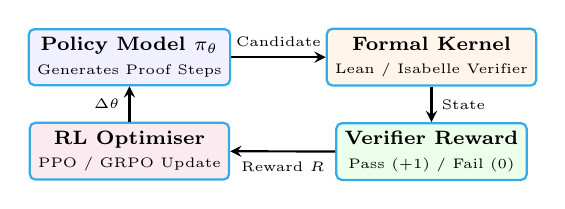
\begin{tikzpicture}[node distance=1.1cm and 1.3cm, auto, >=stealth, thick, font=\scriptsize]
  \node [boxnode, fill=blue!6, minimum width=2.0cm, minimum height=0.6cm, inner sep=3pt] (policy) {\scriptsize \textbf{Policy Model $\pi_\theta$}\\[0.05em] \tiny Generates Proof Steps};
  \node [boxnode, fill=orange!8, right=1.2cm of policy, minimum width=2.0cm, minimum height=0.6cm, inner sep=3pt] (kernel) {\scriptsize \textbf{Formal Kernel}\\[0.05em] \tiny Lean / Isabelle Verifier};
  \node [boxnode, fill=green!8, below=0.45cm of kernel, minimum width=2.0cm, minimum height=0.6cm, inner sep=3pt] (reward) {\scriptsize \textbf{Verifier Reward}\\[0.05em] \tiny Pass (+1) / Fail (0)};
  \node [boxnode, fill=purple!8, below=0.45cm of policy, minimum width=2.0cm, minimum height=0.6cm, inner sep=3pt] (rl) {\scriptsize \textbf{RL Optimiser}\\[0.05em] \tiny PPO / GRPO Update};

  \draw [->] (policy) -- node [above, font=\tiny] {Candidate} (kernel);
  \draw [->] (kernel) -- node [right, font=\tiny] {State} (reward);
  \draw [->] (reward) -- node [below, font=\tiny] {Reward $R$} (rl);
  \draw [->] (rl) -- node [left, font=\tiny] {$\Delta \theta$} (policy);
\end{tikzpicture}

\end{center}

\vspace{-0.3em}
\begin{itemize}
  \item \textbf{Key Players \& Breakthroughs:}
    \begin{itemize}
      \item \textbf{DeepMind} (AlphaProof), \textbf{Harmonic} (Aristotle), \textbf{Axiom Math} (AxiomProver).
      \item \textbf{IMO Gold} achieved in 2025; \textbf{PutnamBench 2025} solved by $\ge 20$ proving systems.
    \end{itemize}
\end{itemize}
\end{frame}

\begin{frame}{3. Democratisation via Agentic Proving}
\note{
\begin{itemize}
  \item Proprietary custom models were extremely expensive and inaccessible to students or individual researchers.
  \item Josef Urban and collaborators discovered that standard, off-the-shelf LLM coding agents are remarkably capable when connected to interactive theorem provers.
  \item In a recent landmark experiment, standard coding agents formalised an entire 800+ theorem textbook on Topology (Munkres) for $\approx \$200$/month.
  \item This connects off-the-shelf agents via Model Context Protocol (MCP) servers, eliminating the multi-million-dollar cost of training custom foundation models.
\end{itemize}
}

\begin{itemize}
  \item \textbf{Inaccessibility of Proprietary Custom Models:}
    \begin{itemize}
      \item Heavy RL infrastructure requires multi-million-dollar compute clusters.
    \end{itemize}
  \vspace{0.5em}
  \item \textbf{Standard Coding Agents + Theorem Prover Loops:}
    \begin{itemize}
      \item Josef Urban showed standard coding agents (e.g.\ \emph{Claude Code}, \emph{Open Code}, \emph{Agy}) can formalise entire textbooks (e.g.\ \emph{Munkres Topology}) for $\approx \$200$/month.
    \end{itemize}
  \vspace{0.5em}
  \item \textbf{Agentic Interactive Workflow:}
    \begin{itemize}
      \item Connects off-the-shelf LLMs directly to provers via Model Context Protocol (MCP).
      \item Eliminates the need for pre-training or fine-tuning custom models.
    \end{itemize}
\end{itemize}
\end{frame}

\begin{frame}{4. Current State \& Industrial Adoption}
\note{
\begin{itemize}
  \item The agentic proving revolution has rapidly transitioned into commercial and industrial application.
  \item Specialised companies have secured significant venture capital funding (e.g.\ Harmonic, Math Inc, Axiom Math).
  \item Major technology companies have adopted formal verification for mission-critical software and hardware systems (e.g.\ AWS, Apple, Arm, Intel).
  \item Top mathematicians like Terence Tao have actively incorporated agentic formal provers into mainstream mathematical research.
\end{itemize}
}

\begin{itemize}
  \item \textbf{Commercial Ecosystem \& Venture Funding:}
    \begin{itemize}
      \item Specialised companies: \emph{Harmonic}, \emph{Math Inc}, \emph{Axiom Math}, etc.\ (securing major VC funding).
    \end{itemize}
  \vspace{0.5em}
  \item \textbf{Industrial Formal Verification:}
    \begin{itemize}
      \item Adoption for mission-critical software \& hardware verification (e.g.\ AWS, Apple, Arm, Intel).
    \end{itemize}
  \vspace{0.5em}
  \item \textbf{Integration in Mathematical Research:}
    \begin{itemize}
      \item Top mathematicians (e.g.\ Terence Tao) incorporating agentic formal provers into active research.
    \end{itemize}
\end{itemize}
\end{frame}

\begin{frame}{5. Technical Setup: Agentic LLMs for Theorem Proving}
\note{
\begin{itemize}
  \item In this week I will demonstrate a new but strongly emerging way to apply theorem provers like Isabelle, via integration with LLMs.
  \item You should have a coding agent ready, e.g.\ Claude Code, Open Code, Codex, Agy, etc.
  \item In my demos I will use Claude Code.
  \item Main idea: Connect a coding agent to the theorem prover via a Model Context Protocol (MCP) server.
  \item An MCP server exposes Isabelle programmatically: write-file, process-file, save-file, etc.
  \item We will use PIDE-MCP (\url{https://github.com/kappelmann/isabelle-pide-mcp}) and AWS's Isabelle/Q (\url{https://github.com/awslabs/AutoCorrode}).
\end{itemize}
}

\begin{itemize}
  \item \textbf{Integrating Theorem Provers with LLMs:}
    \begin{itemize}
      \item Connect a coding agent (e.g.\ \emph{Claude Code}, \emph{Open Code}, \emph{Codex}, \emph{Agy}) directly to Isabelle.
    \end{itemize}
  \vspace{0.5em}
  \item \textbf{Model Context Protocol (MCP) Architecture:}
\end{itemize}

\begin{center}
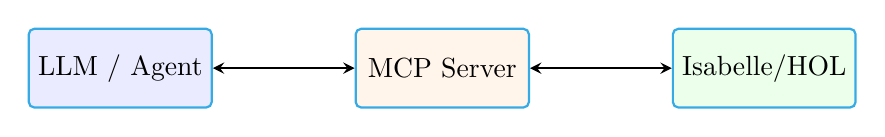
\begin{tikzpicture}[node distance=1.8cm, auto]
  \node [boxnode, fill=blue!8] (llm) {LLM / Agent};
  \node [boxnode, fill=orange!8, right=of llm] (mcp) {MCP Server};
  \node [boxnode, fill=green!8, right=of mcp] (isabelle) {Isabelle/HOL};
  
  \draw [arrow] (llm) -- (mcp);
  \draw [arrow] (mcp) -- (isabelle);
\end{tikzpicture}
\end{center}

\begin{itemize}
  \item \textbf{MCP Implementations \& Repositories:}
    \begin{itemize}
      \item Programmatic actions: \texttt{write-file}, \texttt{process-file}, \texttt{save-file}, etc.
      \item \textbf{PIDE-MCP}: \href{https://github.com/kappelmann/isabelle-pide-mcp}{\textcolor{awesome}{github.com/kappelmann/isabelle-pide-mcp}}
      \item \textbf{Isabelle/Q}: \href{https://github.com/awslabs/AutoCorrode}{\textcolor{awesome}{github.com/awslabs/AutoCorrode}} (AWS Labs)
    \end{itemize}
\end{itemize}
\end{frame}

\begin{frame}{6. Agentic Proving Architectures}
\note{
\begin{itemize}
  \item The most basic agentic architecture for theorem proving consists of a Planner/Sketcher, a Coder, an MCP server, and Isabelle.
  \item Introduced in the "Draft, Sketch, and Prove" paradigm by Jiang, Li et al. \citep{wendaLiSketchProveLLMs}.
  \item The Planner/Sketcher produces detailed proof plans and sketches (e.g.\ sorried proofs).
  \item The Coder takes the proof plans \& sketches, completes them, and ensures Isabelle accepts them via MCP.
  \item If an error cannot be resolved by the Coder, it passes back to the Planner/Sketcher.
  \item Since the area is moving very fast, I will leave a paper on KEATS for you to read and discuss in the LGT.
\end{itemize}
}

\textbf{Basic Two-Stage Agentic Architecture \citep{wendaLiSketchProveLLMs}:}

\begin{center}
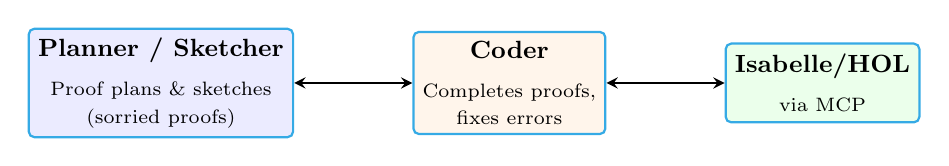
\begin{tikzpicture}[node distance=1.5cm, auto]
  \node [boxnode, fill=blue!8] (planner) {\small \textbf{Planner / Sketcher}\\[0.2em] \scriptsize Proof plans \& sketches\\[-0.2em]\scriptsize (sorried proofs)};
  \node [boxnode, fill=orange!8, right=of planner] (coder) {\small \textbf{Coder}\\[0.2em] \scriptsize Completes proofs,\\[-0.2em]\scriptsize fixes errors};
  \node [boxnode, fill=green!8, right=of coder] (isabelle) {\small \textbf{Isabelle/HOL}\\[0.2em] \scriptsize via MCP};
  
  \draw [arrow] (planner) -- (coder);
  \draw [arrow] (coder) -- (isabelle);
\end{tikzpicture}
\end{center}

\begin{itemize}
  \item \textbf{Workflow \& Feedback Loop (Draft, Sketch \& Prove):}
    \begin{itemize}
      \item Planner creates structured proof sketches (\texttt{sorry}) \citep{wendaLiSketchProveLLMs}.
      \item Coder fills in Isar proof steps \& verifies against Isabelle via MCP.
      \item Unresolved errors loop back from Coder to Planner.
    \end{itemize}
  \vspace{0.2em}
  \item \textbf{Further Reading \& LGT Discussion:}
    \begin{itemize}
      \item As the field is moving very fast, a paper will be provided on \textbf{KEATS} to read and discuss in the \textbf{LGT}.
    \end{itemize}
\end{itemize}
\end{frame}

\begin{frame}{7. Closing Remarks \& Coursework Guidelines}
\note{
\begin{itemize}
  \item You still need to understand technical details yourself: (1) splitting problems, (2) formal modelling, (3) specifications, (4) proving properties (correct, readable/concise, fast checking).
  \item Module Guidelines for LLM use:
    \begin{enumerate}
      \item Design decisions \& proof sketches: Explore alternatives and justify choices.
      \item Proving lower-level facts: Allowed ONLY for facts referencing standard Isabelle distribution definitions. Do NOT use LLMs for facts about your own defined constants.
    \end{enumerate}
  \item Coursework includes a Viva where you must defend your design choices.
  \item Assessment: 50% Coursework (includes Viva) + 50% Exam (paper-based written examination).
\end{itemize}
}

\begin{itemize}
  \item \textbf{Core Skills You Must Master:}
    \begin{enumerate}
      \item Splitting problems into subproblems.
      \item Formally modelling problem domains.
      \item Formulating correct specifications.
      \item Constructing correct, concise, fast-checking proofs (Isabelle linter).
    \end{enumerate}
  \vspace{0.3em}
  \item \textbf{LLM Usage Policy for Coursework:}
    \begin{itemize}
      \item \textbf{Design \& Sketches:} Allowed for exploring design alternatives (must justify choices).
      \item \textbf{Lemma Proving:} Allowed \emph{only} for facts referencing standard library definitions. \textbf{Not allowed} for facts about your own defined constants.
    \end{itemize}
  \vspace{0.3em}
  \item \textbf{Assessment (50\% Coursework + 50\% Exam):}
    \begin{itemize}
      \item \textbf{Coursework (50\%):} Includes a \textbf{Viva} to explain design choices.
      \item \textbf{Exam (50\%):} Paper-based written examination.
    \end{itemize}
\end{itemize}
\end{frame}

\begin{frame}[allowframebreaks]{References}
\bibliographystyle{plainnat}
\bibliography{long_paper}
\end{frame}

\end{document}
